%%\documentclass[binding=0.6cm]{sapthesis}
\documentclass{sapthesis}

\usepackage[english]{babel}
\usepackage[utf8]{inputenc}
\usepackage{graphicx}
\usepackage{float}
\usepackage{hyperref}
\usepackage{algorithm}
\usepackage{algpseudocode}
\usepackage{subcaption}
\usepackage{amssymb}
\usepackage{comment}

\usepackage{caption}
\usepackage{longtable}
\usepackage{listings}
\usepackage{xcolor}
\usepackage{tikz}
\usetikzlibrary{arrows.meta}

\title{Residual Learning for Agile Locomotion: Application to a Two-Wheeled Legged Robot}

\author{Jacopo Tedeschi}
\authoremail{tedeschi.1882789@studenti.uniroma1.it}
\IDnumber{1882789}
\course{Artificial Intelligence and Robotics}
\courseorganizer{Department of Computer, Control and Management Engineering}
\AcademicYear{2025/2026}

\advisor{Prof. Giuseppe Oriolo}
\coadvisor{Prof. Leonardo Lanari}
\coadvisor{Dott. Nicola Scianca}
\thesistype{Master Degree}

%\examdate{January 2027}
\copyyear{2025/2026}

\begin{document}

\maketitle

\begin{abstract}
\
Model-based control and Reinforcement Learning address different limitations in
robotic locomotion. Model Predictive Control (MPC) uses an explicit dynamics
model to optimize future motion and handle physical constraints, but its
performance can degrade when the model does not capture the full behavior of the
system. Reinforcement Learning (RL) can learn behaviors directly through
interaction, making it suitable for compensating for effects that are difficult
to model. However, policies trained from scratch often require extensive reward
design and provide little insight into the resulting control strategy. This
thesis investigates a hybrid approach for the TITA wheeled-legged robot, in
which a learned policy augments a nominal MPC controller instead of replacing
it. The model-based component provides the main control action, while the policy
learns corrections aimed at improving closed-loop performance. The framework
is implemented in JAX using MPX to parallelize the MPC computations required
during training and is evaluated in the MuJoCo physics engine. The evaluation
focuses on the residual controller's behaviour relative to the nominal
model-based controller, with particular attention to tracking accuracy,
robustness, and generalization across different commands and operating
conditions.

\end{abstract}
\clearpage

\tableofcontents

\chapter{Introduction}
Legged robots can traverse environments that remain difficult or inaccessible to
conventional wheeled platforms. Their ability to establish and break contacts
with the ground allows them to negotiate obstacles, uneven surfaces, and
discontinuous terrain. This mobility, however, comes at the cost of a
substantially more complex control problem. Locomotion requires the coordinated
motion of several joints while the robot maintains balance, regulates contact
forces, and tracks the commanded velocity. These objectives must be satisfied
despite impacts, friction uncertainty, actuator limitations, and changes in the
contact configuration.\\
\
Wheeled-legged robots combine articulated limbs with actuated wheels and occupy
an intermediate position between legged and wheeled systems. On regular
surfaces, rolling motion provides greater efficiency and speed than repeated
stepping. When the terrain becomes irregular, the legs can change the height
and orientation of the body, redistribute the contact forces, and step over
obstacles that cannot be crossed through rolling alone. This combination
extends the range of possible motions, but also introduces further control
challenges. The controller must account for the floating-base dynamics, the
unilateral nature of contacts, the rolling constraints of the wheels, and the
interaction between body motion and wheel traction. At higher velocities,
changes in load distribution and imperfect contact modelling can further
reduce stability \cite{racing}.\\
\
Model Predictive Control (MPC) has become one of the main approaches to locomotion
control because it expresses the task as an Optimal Control Problem (OCP). At each
control update, MPC predicts the evolution of the robot over a finite horizon
and computes a sequence of inputs that minimizes a cost function while
satisfying a model of the dynamics and a set of constraints. Only the first
input of the optimized sequence is applied. The optimization is then repeated
from the updated state. This structure allows the controller to consider future
motion rather than reacting only to the current tracking error. It also provides
a direct way to encode objectives such as velocity tracking, body-height regulation, force
distribution, friction limits, and actuator bounds.\\
\
The explicit formulation of the prediction model, objective function, and
constraints makes MPC relatively transparent. Predicted trajectories and
contact forces can be inspected, and individual weights can be adjusted
according to their physical meaning. This is particularly useful in legged
robotics, where controller failures may arise from several interacting sources.
The internal solution provides information that can help distinguish an
infeasible motion request from poor state estimation, incorrect contact
assumptions, or insufficient control authority.\\
\
This structure does not remove the difficulties associated with modelling
locomotion. A full rigid-body model describes the robot more accurately, but
its use over a sufficiently long prediction horizon may be too computationally
expensive for real-time control. Reduced-order models are therefore commonly
adopted. Examples include centroidal models, Single Rigid Body Dynamics models,
and simplified inverted-pendulum representations. These formulations retain
the quantities that dominate the global motion of the robot while omitting part
of the articulated dynamics. The reduction makes online optimization
practical, but creates a discrepancy between predicted and actual behaviour.
Joint dynamics, actuator response, structural compliance, impacts, and complex
wheel--terrain or foot--terrain interactions may only be represented
approximately.\\
\
When a reduced model is used, a Whole-Body Controller (WBC) can be introduced between
the MPC and the actuators. Its purpose is to map the motion quantities and
contact forces planned by MPC to commands that are consistent with the complete
kinematics and dynamics of the robot. A WBC can be formulated as a Quadratic
Programming (QP) problem in which generalized accelerations, contact forces, or joint torques
are selected to track the reduced-order plan. At the same time, the QP can
account for additional requirements that are absent from the simplified MPC
model, including the floating-base equations of motion, friction-cone
conditions, joint limits, contact constraints, swing-foot trajectory tracking,
body-orientation regulation, and posture regularization.  resulting
hierarchy separates long-horizon motion planning from instantaneous whole-body
control. It does not eliminate model mismatch, but it allows several physical
constraints to be enforced without introducing the complete multibody system
into every node of the MPC horizon.\\
\
The performance of the resulting MPC-WBC architecture still depends on the
validity of its models and contact assumptions. Errors in mass and inertia
parameters, terrain height, friction, actuation delay, or contact timing can
produce persistent tracking errors and, in more severe cases, instability.
Some effects can be addressed by increasing model fidelity or adding
constraints and cost terms. This solution is not always practical. A more
detailed formulation increases the computational burden, and some phenomena
are difficult to describe through a compact differentiable model. The
controller therefore faces a persistent compromise between physical accuracy
and the ability to solve the optimization problem at the required frequency.\\
\
Reinforcement Learning (RL) offers a different approach to the same control problem.
Rather than requiring a complete analytical description of the dynamics, an RL
policy learns a mapping from observations to actions through interaction with
an environment. The policy is optimized to maximize the expected cumulative
reward, which can include velocity tracking, stability, energy consumption,
action smoothness, and other task-related objectives. Training under variations
in the robot model, terrain, observations, and external disturbances can
produce behaviours that are less dependent on a single nominal model. RL can
also account implicitly for nonlinear contact effects and objectives that would
be cumbersome to include in an online optimization problem.\\
\
These advantages are accompanied by important limitations. A learned policy
does not normally enforce physical constraints in the explicit form used by
MPC. Its behaviour depends strongly on the training distribution, reward
definition, action representation, and simulation model. Good performance
inside the training domain does not guarantee predictable behaviour in states
that were rarely or never encountered. Reward design can also require
considerable tuning, since a policy may exploit unintended aspects of the
simulator or trade one objective against another in an undesirable way.
Finally, the internal reasoning of a neural policy is difficult to inspect.
Diagnosing a failure is therefore less direct than examining the state,
constraints, and cost terms of a model-based optimizer.\\
\
MPC and RL have complementary strengths. MPC supplies a physically grounded
nominal behaviour, explicit predictions, and structured constraint handling.
RL provides a mechanism for learning corrections from experience when the
nominal model is incomplete. This complementarity has motivated several
combined architectures. A policy may adjust parameters of the optimization
problem, generate reference trajectories or contact schedules, imitate
trajectories produced by an MPC expert, or act in parallel with the model-based
controller \cite{adaptive_mpc,non_gaited}. Each choice
determines how authority is divided between the analytical controller and the
learned component.\\
\
Most established MPC solvers used in robotics are designed primarily for CPU
execution. Although these implementations can achieve the update rates required
to control a single robot, their computational cost becomes a bottleneck when
the controller must be evaluated across thousands of parallel simulation
environments. This requirement is particularly relevant when MPC is included
directly in a Reinforcement Learning training loop. Recent work has therefore
focused on reformulating optimal-control algorithms to exploit Graphics Processing
Unit (GPU) parallelism,
allowing multiple MPC problems to be solved concurrently alongside the learning
process. MPX follows this direction by providing a JAX-based, GPU-accelerated
MPC framework for legged robots \cite{mpx}. Its solver exploits temporal and
state-space parallelism through associative scan operations, enabling the
model-based controller to remain active during large-scale policy training
rather than being used only to generate offline trajectories or reference
motions. Its solver exploits temporal and
state-space parallelism through associative scan operations, reducing the
dependence of computation time on the prediction-horizon length and on the
dimensions of the state and control spaces. Besides supporting real-time
control, this formulation makes it possible to evaluate many MPC instances
concurrently during learning. Model-based control can therefore remain inside
the simulation loop rather than being used only to generate an offline dataset
or a reference trajectory.\\
\
This thesis focuses on residual learning, in which the model-based controller
remains active and the policy produces a correction to its nominal command. The
main locomotion task is therefore not learned from an unstructured initial
policy. MPC and Whole-Body Control provide the nominal motion and the
corresponding actuator torques, while RL learns only the additional contribution
required to improve the closed-loop response. The final command can be
expressed in the general form

$$
\boldsymbol{\tau}_{\mathrm{cmd}}
=
\boldsymbol{\tau}_{\mathrm{nom}}
+
\boldsymbol{\tau}_{\mathrm{res}},
$$

where \(\boldsymbol{\tau}_{\mathrm{nom}}\) is generated by the model-based
control branch and \(\boldsymbol{\tau}_{\mathrm{res}}\) is obtained from the
policy output through a low-level feedback law. The nominal controller provides
a strong control prior and keeps the learning process close to a physically
meaningful locomotion strategy. The policy is then free to compensate for
systematic tracking errors, simplified dynamics, uncertain contacts, and other
effects that are not captured adequately by the nominal formulation. Similar
torque-level residual architectures have shown that an MPC prior can improve
training efficiency and extend the range of trackable locomotion commands
\cite{residual_mpc}.\\
\
The nominal MPC-WBC controller provides a reference for evaluating the effect
of the learned residual correction. When the
learned contribution is bypassed, the robot is controlled by the original architecture. 
When it is enabled, the nominal controller and
experimental conditions remain unchanged, while the policy adds its correction.
The effect of learning can therefore be evaluated without comparing two
entirely different locomotion pipelines.\\
\
The work presented in this thesis studies this approach on the TITA robot
in the MuJoCo physics engine \cite{mujoco}. MuJoCo provides
rigid-body dynamics, contact simulation, and an interface suitable for parallel
learning and control experiments. Both the nominal controllers and the learned
policies are evaluated within the same simulated dynamics, allowing their
behaviour to be compared under consistent initial conditions, velocity
commands, disturbances, and model variations.\\
\
The platform considered in this thesis is TITA, a wheeled-legged robot with two
articulated legs and two actuated wheels. Its nominal MPC is based on the Double Force
Constrained Inverted Pendulum model (DFCIP). This reduced-order
representation describes the quantities that dominate the motion of the robot,
including its centre-of-mass position and velocity, heading, forward velocity,
yaw rate, and wheel contact geometry. From the measured robot state and the
commanded forward and angular velocities, the MPC plans the desired forward,
vertical, and angular accelerations together with the ground reaction forces at
the two wheels.\\
\
These accelerations and ground reaction forces constitute the reduced-order
references supplied by the MPC to the Whole-Body Controller. The WBC formulates
an instantaneous Quadratic Program over the generalized accelerations and wheel
contact forces. Its objective includes tracking tasks for the centre of mass,
the left and right wheels, the base orientation, and the joint posture. The
optimization also accounts for the floating-base equations of motion, friction
constraints, and predicted joint limits. Once the QP has been solved, inverse
dynamics maps the optimized generalized accelerations and contact forces to the
nominal torques of the eight actuators. The WBC therefore connects the
accelerations and ground reaction forces produced by the DFCIP-MPC to the
complete multibody dynamics of TITA.\\
\
For TITA, the residual policy observes the robot state together with selected
outputs of the model-based controller. These include the accelerations and
ground reaction forces planned by MPC and the nominal torques computed by WBC.
The policy therefore has access not only to the measured motion but also to the
action intended by the nominal controller. Its outputs modify the desired
positions of the leg joints and the desired velocities of the wheels.
Joint-level feedback converts these offsets into residual torques, which are
added to the nominal WBC torques before the complete command is applied to the
actuators.\\
\
The objective of this thesis is to determine whether residual learning can
improve the tracking accuracy and robustness of an MPC-based locomotion
controller without discarding its physical structure. The investigation
considers individual and combined velocity commands, stability limits, control
effort, uneven terrain, disturbances, observation noise, and variations in
model parameters. The comparison is not limited to the final tracking error.
It also examines whether improvements are obtained through bounded and
sufficiently smooth corrections, whether the nominal behaviour is preserved
when no correction is needed, and whether the learned component introduces
systematic biases or undesirable interactions with the original controller.\\
\
The main contribution is the development and evaluation of a residual MPC
architecture for TITA. It combines a DFCIP-based MPC, a constrained WBC, and
joint-level residual control on a two-wheeled legged platform. MPC remains
active during policy training and evaluation, allowing the policy to learn
within the same closed-loop architecture used at evaluation and providing a
direct comparison against the unmodified model-based controller. The study
also analyses the practical consequences of residual torque addition,
including action representation, controller update rates, baseline isolation,
and the interaction between the learned and nominal commands.\\
\
The remainder of the thesis develops this investigation from its theoretical
foundations to its experimental evaluation. The next chapter reviews
model-based, learning-based, and hybrid approaches to legged locomotion. The
TITA robot model and its reduced-order representation are then introduced,
followed by the formulation of MPC and Whole-Body Control.
The reinforcement-learning problem, policy observations, actions, and training
procedure are subsequently described. The complete TITA residual architecture
is then presented, including the exchange of information between the
model-based and learned components. Finally, the controller is evaluated in
simulation, the results and limitations are discussed, and the main conclusions
and possible directions for future work are reported.

\clearpage

\chapter{Background and Related Work}
This chapter reviews the main approaches to the control of legged and
wheeled-legged robots, with particular attention to the combination of
model-based control and reinforcement learning. The discussion begins with the
characteristics of these robotic platforms and the challenges introduced by
dynamic locomotion, intermittent contacts, and underactuated floating-base
dynamics.\\
\
Model-based methods are then examined through reduced-order models, Model
Predictive Control, and Whole-Body Control. These techniques provide structured
and interpretable control solutions, but their performance depends on model
accuracy and is constrained by the computational cost of online optimization.
Learning-based locomotion offers a complementary approach, allowing policies to
adapt to complex dynamics and uncertain interactions through experience.\\
\
The chapter subsequently considers hybrid architectures that combine MPC and
Reinforcement Learning. Recent developments in
GPU-accelerated optimal control are discussed, since they make it possible to
execute many MPC instances in parallel and train residual-learning
policies.

\section{Related Works}
\label{sec:related_works}

Optimization-based control has become a standard approach to dynamic legged
locomotion. It formulates motion generation as an Optimal Control Problem
(OCP) in which the robot dynamics, contact forces, physical constraints, and task
objectives are considered explicitly. Solving the complete problem online is
difficult because legged robots have many degrees of freedom and interact with
the environment through intermittent and unilateral contacts
\cite{legged_optimization}. Existing controllers therefore differ in the
dynamic model they employ, the way they represent contacts, and the division of
tasks between predictive planning and low-level control.\\
\
Reduced-order models make online optimization tractable by retaining the
variables that dominate balance and locomotion while neglecting part of the
articulated dynamics. The convex MPC developed for the MIT Cheetah 3 represents
the trunk as a single rigid body and optimizes the ground reaction forces over
a finite horizon \cite{cheetah_mpc}. The whole-body nonlinear MPC of Neunert
et al. instead includes the complete articulated dynamics and explicit contact
dynamics, optimizing robot motion,
contact locations, sequences, and timings within a single problem
\cite{whole_body_nmpc}. This richer representation
reduces the separation between planning and control but results in a more
demanding optimization. Other work has addressed the numerical treatment of
three-dimensional orientation \cite{representation_free_mpc} and adapted solver
accuracy to the time constraints of whole-body locomotion control
\cite{fast_whole_body_mpc}.\\
\
Wheeled-legged robots introduce rolling contacts and additional actuated
degrees of freedom. Early experiments on ANYmal integrated wheel motion and
non-holonomic rolling constraints into a whole-body planning and control
framework \cite{keep_rollin}. Online trajectory optimization was later used to
produce hybrid walking-driving motions on rough terrain
\cite{rolling_deep}. A subsequent whole-body MPC formulation jointly optimize
torso motion, wheel motion, and contact forces using a kinodynamic model that
combines Single Rigid Body Dynamics with whole-body kinematics. Unlike the
full-dynamics formulation discussed above, this model does not retain the
complete articulated dynamics. A separate gait-sequence generator uses
kinematic leg utilities to adapt contact timings online
\cite{wheeled_whole_body_mpc}. These approaches coordinate wheel motion with
leg configuration, body dynamics, and contact forces rather than treating the
wheels as an independent drivetrain.\\
\
The wheeled-legged studies discussed above focus on terrain traversal and the
transition between rolling and stepping. At higher speeds, vehicle-like
effects become increasingly relevant. In particular, lateral load transfer
during cornering can unload the inner wheels and bring the robot closer to
rollover \cite{racing}. A recent controller for the Unitree
Go2-W combined an MPC planner for active roll regulation with a learned
low-level policy. The legs were used as an active suspension system to lean the
body into turns and reduce lateral load transfer during physical racing
experiments \cite{racing}.\\
\
Reinforcement Learning provides a different approach to the uncertainties and
contact interactions involved in locomotion. Policies trained in simulation
have been transferred to physical quadrupeds for agile movements and locomotion
over challenging terrain \cite{agile_motor_skills,challenging_terrain}.
Perceptive policies have also demonstrated locomotion in natural environments
using proprioceptive and exteroceptive information
\cite{perceptive_rl}. These methods can learn behaviours that are difficult to
describe through an analytical model, but their performance depends on the
training distribution, reward formulation, observation design, and simulation
accuracy.\\
\
The computational structure of RL has encouraged massively parallel
simulation. Thousands of robots can be simulated simultaneously on a
GPU,
producing large batches of experience for policy optimization. This approach
has substantially reduced the time required to train locomotion policies and
supports curriculum learning across many parallel environments
\cite{parallel_rl}. A purely model-free policy, however, does not explicitly
encode the physical constraints or the structure available to an
optimization-based controller. This limitation has motivated methods that
combine learning and model-based control.\\
\
Some hybrid architectures combine a model-based motion planner with an RL
policy trained to execute the planned motion. In \cite{deep_tracking},
trajectory optimization generates footholds and base motion and, during training,
rewards encourage base-motion tracking and accurate foot placement, while the
actor observes selected planning outputs rather than the full optimized base
trajectory. The planner remains active during deployment.
Lee et al. instead use Linear Inverted Pendulum dynamics
to generate desired foot placements from velocity commands. Their RL policy
tracks those placements without being required to follow the complete motion
predicted by the reduced model \cite{footstep_rl}. In both cases, the model
guides the learned behaviour, while the policy remains responsible for
producing the low-level control action.\\
\
Hierarchical methods  can also assign high-level decisions to RL and motion generation
to MPC, reversing the roles of the model-based and learned components in the
preceding examples. In
\cite{non_gaited}, a high-level RL policy selects acyclic contact patterns and
navigation commands for a low-level MPC. This removes the combinatorial search
over contact sequences from the continuous optimization and allows the same
architecture to address legged and hybrid wheeled-legged locomotion.\\
\
Other approaches use learning to adapt the prediction model or individual
components of the nominal control architecture. Learned corrections have been introduced
to reduce the
discrepancy between reduced-order predictions and the full-order dynamics of a
quadruped \cite{model_gap}. Modular residual methods apply learned corrections
to individual parts of a model-based controller, including its dynamics model
and footstep planner \cite{modular_residual}. In the adaptive architecture
presented in \cite{adaptive_mpc}, RL modifies the predictive dynamics, the
swing-leg controller, and the gait frequency. These adaptations affect both
the MPC problem and the generation of swing-leg commands, rather than adding
a residual torque to the nominal actuator command.\\
\
Residual corrections can therefore act inside the model-based architecture,
as in the model and planner adaptations discussed above. Action-level residual
policy learning instead applies the correction to the nominal control output. A
conventional
controller supplies a nominal action, while RL learns only the correction
needed to improve the resulting behaviour. This approach has been demonstrated
in contact-rich manipulation tasks, where a feedback controller captured the
known structure and a residual policy compensated for effects that were
difficult to model \cite{residual_robot_control}. For locomotion, corrections
to joint setpoints and corrections expressed directly as torques provide
different ways of modifying the nominal actuator command
\cite{residual_mpc}.\\
\
The work most closely related to this thesis is Residual MPC, which executes an
MPC controller and a residual policy concurrently and combines their outputs at
the torque-control level \cite{residual_mpc}. The MPC provides a structured
control prior, while the policy learns corrections for modelling errors and
behaviours that are difficult to encode in the optimization. The paper compares
different residual action spaces and torque-blending strategies, showing that
the action representation and the way the outputs are combined affect both
learning and final locomotion behaviour \cite{residual_mpc}. Unlike approaches based on
offline demonstrations, MPC
remains active during training and deployment.\\
\
This integration creates a substantial computational requirement. An MPC
problem must be solved for every simulated robot at each control update.
Optimal-control solvers for legged locomotion have traditionally been designed
for sequential execution on Central Processing Units
(CPUs), whereas modern RL environments simulate
thousands of agents in parallel on GPUs. The resulting separation between CPU
optimization and GPU training limits the number of MPC instances that can be
kept inside the learning loop \cite{residual_mpc,mpx}.\\
\
CusADi addressed this problem by translating symbolic expressions into
GPU-compatible operations and evaluating large batches of approximate
optimal-control problems in parallel \cite{cusadi}. ReLU-QP addresses the
solution of quadratic programs by expressing Alternating Direction Method of
Multipliers (ADMM) iterations as a weight-tied
network with ReLU activations, allowing execution through standard
machine-learning tools on GPUs \cite{relu_qp}. MPX uses a primal-dual
iterative Linear Quadratic Regulator (iLQR) formulation
implemented in JAX. Associative scans enable temporal and state-space
parallelization, while batching supports many independent MPC instances on
the same device \cite{mpx}. This enables MPC to remain directly inside a
massively parallel RL training loop.\\
\
These studies motivate the combination of a model-based locomotion controller
with learned corrections, but their models and control hierarchies cannot be
transferred unchanged to TITA. The robot shares the rolling-contact constraints
of wheeled quadrupeds, while its two-wheel support makes body balance and the
coordination of wheel traction with leg motion central to the control problem.
This thesis adopts the action-level residual approach: a DFCIP-based MPC and a
constrained Whole-Body Controller generate the nominal command, while the
policy modifies torque-level references to produce an additional torque
contribution. The MPC and WBC remain active during training. Compared with the
kinodynamic whole-body MPC used in Residual MPC \cite{residual_mpc}, the TITA
architecture separates reduced-order prediction from whole-body torque
computation. The architecture chapter describes this decomposition and how
the learned correction is combined with the nominal command.


\newpage
\section{Legged and Wheeled-Legged Locomotion}
\label{sec:legged_wheeled_legged_locomotion}

Legged robots move through the environment directly through force contacts
exchange with the surrounding terrain. Unlike conventional wheeled
vehicles, they do not require a continuous and approximately flat path. Each
foot can be placed on a separate support surface, allowing the robot to cross
steps, gaps, debris, and other irregular terrain. This mobility makes legged
systems suitable for environments in which fixed infrastructure is unavailable
or ordinary vehicles cannot operate \cite{legged_optimization}.\\
\
This capability introduces a demanding control problem. A legged robot is a
floating-base mechanical system whose body is not directly actuated. Its motion
must be generated indirectly through the forces exchanged at the active
contacts. These contacts change during locomotion and are governed by
unilateral and friction constraints: a foot can push against the terrain but
cannot pull on it, while excessive tangential force may cause slipping. The
controller must coordinate joint motion, contact timing, and ground reaction
forces while maintaining balance and tracking the desired movement
\cite{legged_optimization}.\\
\
The complexity of locomotion also depends on the selected gait. Periodic gaits,
such as walking, trotting, and bounding, define recurring sequences of stance
and swing phases. During stance, the contacting limbs support and accelerate
the body. During swing, the remaining limbs are repositioned for the next
contact. Faster motions reduce the time available for feedback and may include
phases with a small support region or no ground contact. Aperiodic locomotion
provides more freedom to react to the terrain, but selecting contact timings
while planning the continuous motion makes the control problem considerably
harder \cite{legged_optimization,non_gaited}.\\
\
Model uncertainty further separates the predicted and actual motion. Impacts,
actuator limitations, delayed measurements, uncertain friction, and imperfect
terrain information cannot always be represented accurately. These effects are
particularly important when a controller relies on a reduced-order model, since
the neglected articulated dynamics still influence the physical robot. Robust
locomotion therefore requires continuous feedback and repeated adaptation of
the planned motion.\\
\
Wheeled-legged robots extend this mobility by placing wheels at the ends of
some or all limbs. On regular terrain, rolling avoids the repeated
acceleration and deceleration associated with conventional stepping and can
provide faster and more energy-efficient locomotion
\cite{wheeled_legged_survey,keep_rollin}. When the terrain becomes
discontinuous or unsuitable for rolling, the articulated legs can adjust the
body posture, negotiate obstacles, or initiate a stepping motion
\cite{rolling_deep}. The same platform can therefore use rolling for efficient
traversal and leg motion when the geometry of the environment requires it.\\
\
The mechanical arrangement of the wheels determines the available mobility.
Some platforms use steerable wheels, whereas others mount non-steerable wheels
at the ends of the legs. In the latter case, each contact can move along the
rolling direction but should not slide laterally. The controller must enforce
this non-holonomic condition while coordinating wheel velocity, leg
configuration, body motion, and contact forces
\cite{keep_rollin,wheeled_whole_body_mpc}. The wheels increase the set of
feasible motions, but also couple locomotion and posture control more tightly
than in a purely legged system.\\
\
Wheeled-legged locomotion can be divided into rolling, stepping, and hybrid
motions. During rolling, the wheels remain in contact with the ground and the
legs regulate the posture of the body. During stepping, one or more wheel
contacts are lifted and repositioned as ordinary feet. Hybrid locomotion
combines these modes within the same manoeuvre, allowing the robot to drive
across traversable regions and step over local obstacles
\cite{rolling_deep}. The contact sequence may be prescribed in advance or
adapted online according to the state of the robot and its kinematic limits
\cite{wheeled_whole_body_mpc}.\\
\
The addition of wheels does not remove the difficulties associated with legged
locomotion. Rolling contacts introduce further constraints, and transitions
between driving and stepping modify the support configuration. At higher
speeds, acceleration and cornering also redistribute the normal loads between
the contacts. This lateral load transfer reduces the available contact margin
and can increase the risk of wheel slip or rollover. On skid-steered platforms,
yaw is generated through differential wheel torques, further coupling
longitudinal motion, lateral dynamics, and body posture \cite{racing}.\\
\
Articulated legs can be used to mitigate these effects. By changing the
relative extension of the legs on either side of the body, a wheeled-legged
robot can regulate its roll angle and redistribute the contact loads. Physical
experiments on the Unitree Go2-W demonstrated this principle by using the legs
as an active suspension system and leaning the body into turns
\cite{racing}. This extends the role of the legs beyond obstacle traversal:
their configuration also affects stability and vehicle-like dynamics during
fast rolling.\\
\
Legged and wheeled-legged robots thus share the need to regulate an
underactuated floating body through constrained ground contacts. Wheels improve
continuous mobility on suitable terrain, but introduce rolling constraints,
additional actuation, and high-speed effects that are absent or less prominent
in conventional stepping. These properties motivate controllers that can plan
body motion and contact forces online while remaining sufficiently efficient
for closed-loop operation.


\newpage
\section{GPU-Accelerated Optimization and Learning}



\clearpage

\chapter{Model-Based Locomotion Control}
\label{sec:model_based_control}

Predicting the full floating-base dynamics over a long horizon can be expensive
for real-time control. Model-based locomotion controllers therefore use two
layers \cite{legged_optimization, cheetah_mpc}. An MPC plans the motion of the
centre of mass and the contact forces on a reduced-order model. A Whole-Body
Controller then turns this plan into joint torques, using the full dynamics and
the actuator limits.\\
\
The TITA controller has the same structure.
Section~\ref{subsec:dfcip_mpc} presents the DFCIP-based MPC, and
Section~\ref{subsec:wbc_dfcip} presents the WBC.


\section{Double Forces Constrained Inverted Pendulum MPC}
\label{subsec:dfcip_mpc}

The predictive controller used for TITA is based on the Double Forces
Constrained Inverted Pendulum (DFCIP). The model describes the centre of mass
as a point mass supported by two ground reaction forces, one for each wheel.
The motion of the wheeled support is represented by a virtual unicycle located
at the midpoint between the wheel contacts.\\
\
Figure~\ref{fig:dfcip_model} shows how the model sits on top of the real robot.
The red point is the CoM whose dynamics depend on the forces 
which came from the wheel contacts.
%
\begin{figure}[H]
    \centering
    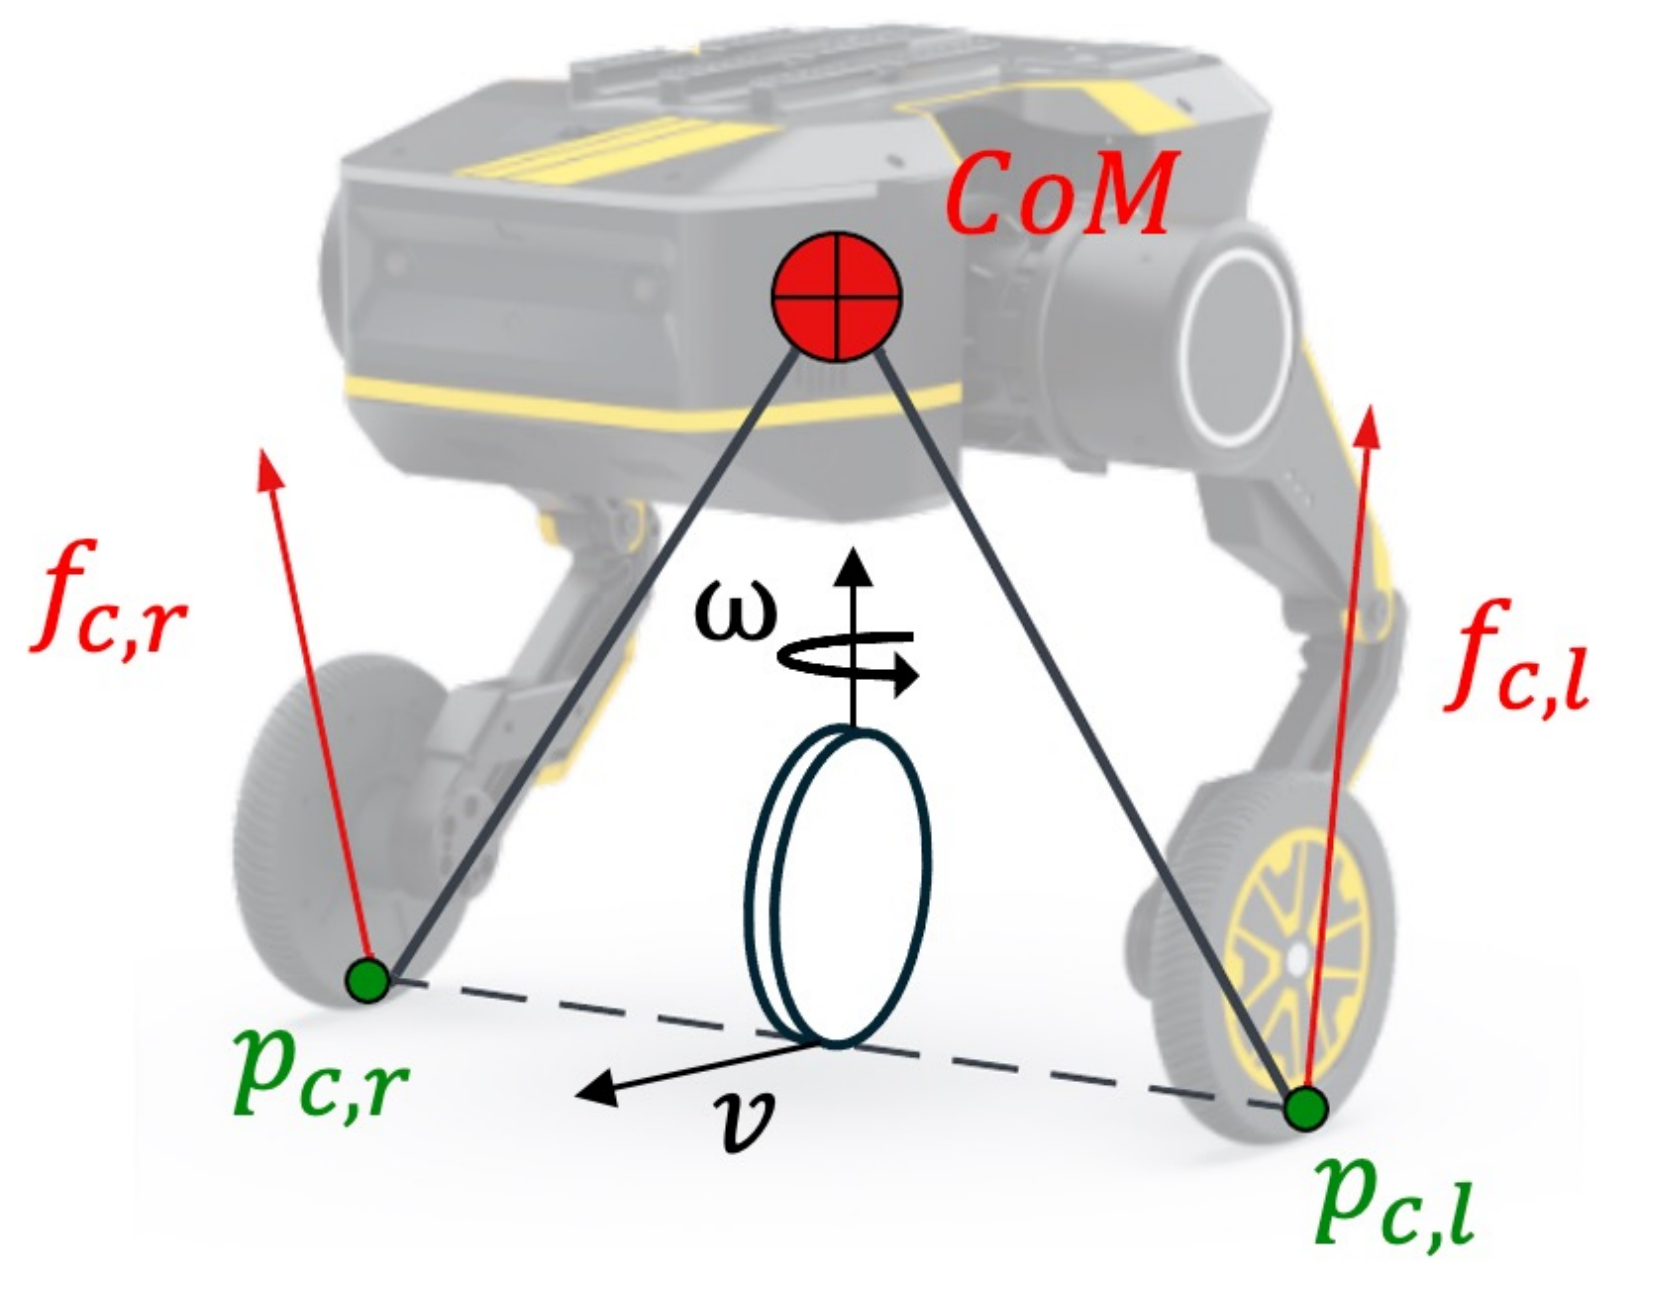
\includegraphics[width=0.6\textwidth]{images/dfcip_model.png}
    \caption{DFCIP template model overlaid on TITA. The CoM is a point mass
    supported by the contact forces \(f_{c,l}\) and \(f_{c,r}\) (denoted
    \(\mathbf{F}_L\) and \(\mathbf{F}_R\) in the text), applied at the wheel
    contacts \(p_{c,l}\) and \(p_{c,r}\). The virtual unicycle at their
    midpoint moves with forward speed \(v\) and yaw rate \(\omega\).}
    \label{fig:dfcip_model}
\end{figure}
%
\noindent The DFCIP state is
\begin{equation}
    \mathbf{x}
    =
    \begin{bmatrix}
        \mathbf{p}_{\mathrm{CoM}}^{\top} &
        \mathbf{v}_{\mathrm{CoM}}^{\top} &
        \mathbf{c}^{\top} &
        v_{c,z} &
        \theta &
        v &
        \omega
    \end{bmatrix}^{\top}
    \in\mathbb{R}^{13},
    \label{eq:dfcip_state}
\end{equation}
%
where $\mathbf{p}_{\mathrm{CoM}}$ and $\mathbf{v}_{\mathrm{CoM}}$ are the
centre-of-mass position and velocity. The vector $\mathbf{c}$ denotes the
midpoint between the two wheel contacts, while $v_{c,z}$ is its vertical
velocity. The heading angle, forward speed, and yaw rate of the virtual
unicycle are denoted by $\theta$, $v$, and $\omega$.\\
\
At each update, MPC optimizes a sequence of control inputs
$U = (\mathbf{u}_0, \ldots, \mathbf{u}_{N-1})$ over the prediction
horizon with the form
%
\begin{equation}
    \mathbf{u}
    =
    \begin{bmatrix}
        a &
        a_{c,z} &
        \alpha &
        \mathbf{F}_{L}^{\top} &
        \mathbf{F}_{R}^{\top}
    \end{bmatrix}^{\top}
    \in\mathbb{R}^{9}.
    \label{eq:dfcip_input}
\end{equation}
%
The first element, $\mathbf{u}_0$ of the optimized control sequence, is used to construct the WBC
references. The control components are the forward, angular and vertical acceleration
of the CoM, and the ground reaction forces applied to the wheel contact points.
\
The centre-of-mass dynamics are
%
\begin{equation}
    \dot{\mathbf{p}}_{\mathrm{CoM}}
    =
    \mathbf{v}_{\mathrm{CoM}},
    \qquad
    \dot{\mathbf{v}}_{\mathrm{CoM}}
    =
    \mathbf{g}
    +
    \frac{1}{m}
    \left(
        \mathbf{F}_{L}
        +
        \mathbf{F}_{R}
    \right).
    \label{eq:dfcip_com_dynamics}
\end{equation}
%
The midpoint between the wheel contacts follows the unicycle dynamics
%
\begin{equation}
\begin{aligned}
    \dot{c}_x
        &=
        v\cos\theta, &
    \dot{c}_y
        &=
        v\sin\theta, \\
    \dot{c}_z
        &=
        v_{c,z}, &
    \dot{v}_{c,z}
        &=
        0, \\
    \dot{\theta}
        &=
        \omega, &
    \dot{v}
        &=
        a, \qquad
    \dot{\omega}
        =
        \alpha.
\end{aligned}
\label{eq:dfcip_unicycle_dynamics}
\end{equation}
%
The equations for $\dot{c}_x$ and $\dot{c}_y$ enforce the nonholonomic
structure of the wheeled base: the support midpoint moves along the direction
defined by $\theta$ and has no independent lateral-velocity input. The model is
discretized using forward Euler integration with prediction time step
$dt_{\mathrm{mpc}}$.\\
\
Let $d$ denote the distance between the wheels. Their contact positions are
reconstructed from the midpoint and heading:
%
\begin{equation}
\begin{aligned}
    \mathbf{p}_{c,L}
        &=
        \mathbf{c}
        +
        \mathbf{R}_{z}(\theta)
        \begin{bmatrix}
            0 & d/2 & 0
        \end{bmatrix}^{\top}, \\
    \mathbf{p}_{c,R}
        &=
        \mathbf{c}
        -
        \mathbf{R}_{z}(\theta)
        \begin{bmatrix}
            0 & d/2 & 0
        \end{bmatrix}^{\top}.
\end{aligned}
\label{eq:dfcip_contact_positions}
\end{equation}
%
Since the DFCIP does not include an explicit rotational state for the complete
robot, a moment constraint is introduced to ensure the balance
%
\begin{equation}
    \mathbf{r}_{M,k}
    =
    \left(
        \mathbf{p}_{c,L,k}
        -
        \mathbf{p}_{\mathrm{CoM},k}
    \right)
    \times
    \mathbf{F}_{L,k}
    +
    \left(
        \mathbf{p}_{c,R,k}
        -
        \mathbf{p}_{\mathrm{CoM},k}
    \right)
    \times
    \mathbf{F}_{R,k}.
    \label{eq:dfcip_moment_residual}
\end{equation}
%
Penalizing this residual couples the location of the centre of mass to the
left--right force distribution. During turning, for example, the optimizer can
vary the tangential and vertical components of the two forces while limiting
the unmodelled resultant moment.\\
\
The DFCIP objective contains a larger set of possible tracking residuals. The stage cost is
%
\begin{equation}
\begin{aligned}
    \ell_k = 
        &w_{p_{xy}}
        \left(
            p_{\mathrm{CoM},xy,k}
            -p_{\mathrm{CoM},xy,k}^{\mathrm{ref}}
        \right)^2
        +w_{p_z}
        \left(
            p_{\mathrm{CoM},z,k}
            -p_{\mathrm{CoM},z,k}^{\mathrm{ref}}
        \right)^2
        \\
        &+w_{v_{xy}}
        \left(
            v_{\mathrm{CoM},xy,k}
            -v_{\mathrm{CoM},xy,k}^{\mathrm{ref}}
        \right)^2
        +w_{v_z}
        \left(
            v_{\mathrm{CoM},z,k}
            -v_{\mathrm{CoM},z,k}^{\mathrm{ref}}
        \right)^2
        \\
        &+w_c\left(c_k-c_k^{\mathrm{ref}}\right)^2
        +w_{v_c}
        \left(v_{c,z,k}-v_{c,z,k}^{\mathrm{ref}}\right)^2
        +w_{\theta}
        \left(\theta_k-\theta_k^{\mathrm{ref}}\right)^2
        \\
        &+w_v\left(v_k-v_k^{\mathrm{ref}}\right)^2
        +w_{\omega}\left(\omega_k-\omega_k^{\mathrm{ref}}\right)^2
        \\
        &+w_a\left(a_k-a_k^{\mathrm{ref}}\right)^2
        +w_{a_z}
        \left(a_{c,z,k}-a_{c,z,k}^{\mathrm{ref}}\right)^2
        +w_{\alpha}
        \left(\alpha_k-\alpha_k^{\mathrm{ref}}\right)^2
        \\
        &+\sum_{i\in\{L,R\}}
        \left[
            w_{F_{xy}}
            \left(F_{i,xy,k}-F_{i,xy,k}^{\mathrm{ref}}\right)^2
            +w_{F_z}
            \left(F_{i,z,k}-F_{i,z,k}^{\mathrm{ref}}\right)^2
        \right]
        \\
        &+w_{\mathrm{eq}}
        \left[
            v_{c,z,k}^{2}
            +r_{M,k}
            +\sum_{i\in\{L,R\}}
             \min\left(F_{i,z,k},0\right)^2
        \right]
\end{aligned}
\label{eq:dfcip_stage_cost}
\end{equation}
%
Where momentum is expressed as 
%
\begin{equation}
    r_{F_z,k}
    =
    \min\left(F_{L,z,k},0\right)^2
    +
    \min\left(F_{R,z,k},0\right)^2.
    \label{eq:dfcip_unilateral_force}
\end{equation}
%
It is zero when both vertical forces are nonnegative and increases when either
wheel force would pull on the ground. The residual $v_{c,z,k}^{2}$ keeps the
virtual wheel midpoint on the flat contact surface. These relations are
treated as soft constraints through the large coefficient
$w_{\mathrm{eq}}$.\\
\
The reference generator assigns
%
\begin{equation}
\begin{aligned}
    p_{\mathrm{CoM},z}^{\mathrm{ref}}
        &= z_{\mathrm{target}}, \\
    v_{\mathrm{CoM},z}^{\mathrm{ref}}
        &= 0, \\
    v_{c,z}^{\mathrm{ref}}
        &= 0, \\
    \mathbf{F}_{L}^{\mathrm{ref}}
        &=
        \begin{bmatrix}
            0 & 0 & mg/2
        \end{bmatrix}^{\top}, \\
    \mathbf{F}_{R}^{\mathrm{ref}}
        &=
        \begin{bmatrix}
            0 & 0 & mg/2
        \end{bmatrix}^{\top}.
\end{aligned}
\label{eq:dfcip_nominal_references}
\end{equation}
%
The desired forward speed and yaw rate are approached through
acceleration-limited profiles. At each prediction step,
%
\begin{equation}
\begin{aligned}
    v_{k+1}^{\mathrm{ref}}
        &=
        v_k^{\mathrm{ref}}
        +
        \operatorname{clip}
        \left(
            v^{\mathrm{cmd}}-v_k^{\mathrm{ref}},
            -a_{\max}\Delta t,
            a_{\max}\Delta t
        \right), \\
    \omega_{k+1}^{\mathrm{ref}}
        &=
        \omega_k^{\mathrm{ref}}
        +
        \operatorname{clip}
        \left(
            \omega^{\mathrm{cmd}}-\omega_k^{\mathrm{ref}},
            -\alpha_{\max}\Delta t,
            \alpha_{\max}\Delta t
        \right).
\end{aligned}
\label{eq:dfcip_velocity_ramp}
\end{equation}
%
The planar centre-of-mass velocity reference is aligned with the predicted
heading:
%
\begin{equation}
    \mathbf{v}_{\mathrm{CoM},xy,k}^{\mathrm{ref}}
    =
    v_k^{\mathrm{ref}}
    \begin{bmatrix}
        \cos\theta_k^{\mathrm{ref}} \\
        \sin\theta_k^{\mathrm{ref}}
    \end{bmatrix}.
    \label{eq:dfcip_com_velocity_reference}
\end{equation}
%
The objective therefore tracks forward speed in two related forms: through the
scalar unicycle speed $v$ and through the planar centre-of-mass velocity. The
first represents the motion of the wheel midpoint along its heading, whereas
the second regulates the global translational motion of the centre of mass.\\
\
At the terminal node, input-dependent terms are removed and an additional
stability residual is introduced:
%
\begin{equation}
    \mathbf{r}_{\mathrm{stab},N}
    =
    \mathbf{p}_{\mathrm{CoM},xy,N}
    -
    \mathbf{c}_{xy,N}.
    \label{eq:dfcip_terminal_stability}
\end{equation}
%
The terminal cost is
%
\begin{equation}
\begin{aligned}
    \ell_N =
        &w_{p_{xy}}
        \left(
            p_{\mathrm{CoM},xy,N}
            -p_{\mathrm{CoM},xy,N}^{\mathrm{ref}}
        \right)^2
        +w_{p_z}
        \left(
            p_{\mathrm{CoM},z,N}
            -p_{\mathrm{CoM},z,N}^{\mathrm{ref}}
        \right)^2
        \\
        &+w_{v_{xy}}
        \left(
            v_{\mathrm{CoM},xy,N}
            -v_{\mathrm{CoM},xy,N}^{\mathrm{ref}}
        \right)^2
        +w_{v_z}
        \left(
            v_{\mathrm{CoM},z,N}
            -v_{\mathrm{CoM},z,N}^{\mathrm{ref}}
        \right)^2
        \\
        &+w_c
        \left(
            c_N-c_N^{\mathrm{ref}}
        \right)^2
        +w_{v_c}
        \left(
            v_{c,z,N}-v_{c,z,N}^{\mathrm{ref}}
        \right)^2
        +w_{\theta}
        \left(
            \theta_N-\theta_N^{\mathrm{ref}}
        \right)^2
        \\
        &+w_v
        \left(
            v_N-v_N^{\mathrm{ref}}
        \right)^2
        +w_{\omega}
        \left(
            \omega_N-\omega_N^{\mathrm{ref}}
        \right)^2
        \\
        &+w_{\mathrm{eq}}
        \left[
            v_{c,z,N}^{2}
            +\left(
                p_{\mathrm{CoM},xy,N}-c_{xy,N}
            \right)^2
        \right]
\end{aligned}
\label{eq:dfcip_terminal_cost}
\end{equation}
%
The terminal condition encourages the centre-of-mass projection to return over
the midpoint of the two wheels. It acts as a reduced stability objective at the
end of the finite horizon. Moment balance and unilateral-force penalties are
stage terms and are not included in the implemented terminal cost.\\
\
The tasks solved directly by the TITA DFCIP-MPC are:

\begin{itemize}
    \item regulating the centre-of-mass $p_{\mathrm{CoM}}$;
    \item tracking the centre-of-mass velocity $v_{\mathrm{CoM}}$;
    \item tracking the forward speed of the wheeled support $v$;
    \item tracking the commanded yaw rate $\omega$;
    \item regularizing forward, vertical, and yaw accelerations $a$, $a_{c,z}$, $\alpha$;
    \item distributing the ground reaction forces between the two wheels $\mathbf{F}_L$, $\mathbf{F}_R$;
    \item regularizing tangential and vertical contact forces around their nominal references $F_{i,xy}$, $F_{i,z}$;
    \item enforcing moment balance through a soft residual $r_M$;
    \item maintaining zero vertical velocity of the wheel midpoint $v_{c,z}$;
    \item penalizing negative wheel normal forces $F_{i,z}<0$;
\end{itemize}
\
Planar centre-of-mass position, the position of the virtual contact midpoint,
its vertical-velocity reference, and the absolute heading angle appear in the
general objective implementation but have zero weight in the configuration
used for this work.\\
\
The controller assumes permanent contact with flat ground. It does not
switch between stance and flight dynamics, and the contact forces are not set
to zero during any part of the prediction.\\
\
The DFCIP-MPC plans the motion of a reduced model; it does not enforce the
articulated robot's equations of motion or joint-level limits. Its contact
forces are therefore a prediction, not yet a dynamically feasible motor
command. The Whole-Body Controller (WBC) receives the first MPC control and
the measured robot state, then computes joint torques while enforcing
whole-body dynamics, rolling, friction, and joint-limit constraints
(Section~\ref{subsec:wbc_dfcip}).\\
\
For TITA, the prediction horizon contains $N$ intervals of duration
$dt_{\mathrm{mpc}}$, giving a total horizon $T = N\,dt_{\mathrm{mpc}}$.
The MPC is updated at frequency $f_{\mathrm{mpc}}$, with
$n_{\mathrm{iter}}$ solver iterations per update. The previous solution is
shifted to initialize the next OCP. The same reduced-order problem is solved
independently for each simulated environment through the batched GPU
implementation provided by MPX \cite{mpx}.

\begingroup
\small
\setlength{\tabcolsep}{4pt}
\begin{longtable}{p{0.62\textwidth} p{0.28\textwidth}}
\caption{TITA DFCIP-MPC parameters and objective weights.}
\label{tab:tita_mpc_parameters}\\
\hline
\textbf{Parameter} & \textbf{Value} \\
\hline
\endfirsthead
\hline
\textbf{Parameter} & \textbf{Value} \\
\hline
\endhead
\hline
\endfoot
\hline
\endlastfoot
\multicolumn{2}{l}{\textbf{Prediction and reduced-order model}}\\
MPC update frequency, $f_{\mathrm{mpc}}$ & 100 Hz\\
Prediction timestep, $\Delta t_{\mathrm{mpc}}$ & 0.01 s\\
Horizon length, $N$ & 50 intervals\\
Prediction horizon, $T$ & 0.5 s\\
FDDP iterations per update, $n_{\mathrm{iter}}$ & 1\\
State dimension, $n_x$ & 13\\
Control dimension, $n_u$ & 9\\
Robot mass, $m$ & 27.6898 kg\\
Wheel-contact separation, $d$ & 0.567 m\\
Gravity, $g$ & 9.81 m/s$^2$\\
\multicolumn{2}{l}{\textbf{State and input cost weights}}\\
CoM planar position, $w_{p_{xy}}$ & 0\\
CoM height, $w_{p_z}$ & $2\times10^{4}$\\
CoM planar velocity, $w_{v_{xy}}$ & $3\times10^{2}$\\
CoM vertical velocity, $w_{v_z}$ & $1\times10^{1}$\\
Wheel-midpoint position, $w_c$ & 0\\
Wheel-midpoint vertical velocity, $w_{v_c}$ & 0\\
Heading, $w_\theta$ & 0\\
Forward speed, $w_v$ & $1\times10^{1}$\\
Yaw rate, $w_\omega$ & 5\\
Forward acceleration, $w_a$ & $1\times10^{-1}$\\
Vertical acceleration, $w_{a_z}$ & $1\times10^{-1}$\\
Yaw acceleration, $w_\alpha$ & $1\times10^{-3}$\\
Horizontal contact force, $w_{F_{xy}}$ & $1\times10^{-7}$\\
Vertical contact force, $w_{F_z}$ & $1\times10^{-4}$\\
Soft-constraint penalty, $w_{\mathrm{eq}}$ & $1\times10^{6}$\\
\end{longtable}
\endgroup



\newpage
\section{Whole-Body Control}
\label{subsec:wbc_dfcip}
The WBC used for TITA turns the reduced-order MPC plan into joint torques by
solving a quadratic program (QP) over the full robot model. Its decision vector
contains generalized accelerations and the three-dimensional forces at the
left and right wheel contacts,
\[
    x = \begin{bmatrix}
        \ddot{q}^{\top} & f_L^{\top} & f_R^{\top}
    \end{bmatrix}^{\top},
    \qquad \ddot{q}\in\mathbb{R}^{n_v},
\]
where $n_v=6+n_j$ counts the six floating-base velocities and the $n_j$
actuated joints ($n_j=8$ for TITA).
The QP computes generalized accelerations and wheel contact forces while
imposing the floating-base equations of motion as equality constraints. The
actuator torques are then calculated from the optimized accelerations and
contact forces using inverse dynamics.\\
The desired WBC references are constructed from the first control input
$u_0$ of the optimized MPC sequence and the current robot state:
CoM position, velocity, and acceleration; left and right wheel trajectories;
and base yaw, angular velocity, and angular acceleration. These references
form the feedforward and PD terms of the commanded task accelerations. Joint
posture is referenced to the nominal configuration, with zero reference joint
velocity and acceleration. The whole-body QP minimizes the following weighted
quadratic cost:
\begin{equation}
\begin{aligned}
H_{\mathrm{WBC}}(x) ={}&
    w_{\mathrm{com}}
    \left\|J_{\mathrm{com}}\ddot{q}
        +\dot{J}_{\mathrm{com}}\dot{q}
        -a_{\mathrm{com}}^{\mathrm{cmd}}\right\|^2
    \\
    &+w_{\mathrm{lw}}
    \left\|J_{\mathrm{lw}}\ddot{q}
        +\dot{J}_{\mathrm{lw}}\dot{q}
        -a_{\mathrm{lw}}^{\mathrm{cmd}}\right\|^2
    +w_{\mathrm{rw}}
    \left\|J_{\mathrm{rw}}\ddot{q}
        +\dot{J}_{\mathrm{rw}}\dot{q}
        -a_{\mathrm{rw}}^{\mathrm{cmd}}\right\|^2
    \\
    &+w_{\mathrm{base}}
    \left\|J_{\mathrm{base}}^{\omega}\ddot{q}
        +\dot{J}_{\mathrm{base}}^{\omega}\dot{q}
        -\alpha_{\mathrm{base}}^{\mathrm{cmd}}\right\|^2
    \\
    &+w_{\mathrm{posture}}
    \left\|S\left(\ddot{q}
    -a_{\mathrm{posture}}^{\mathrm{cmd}}\right)\right\|^2
    +w_{\ddot{q}}\|\ddot{q}\|^2
    +\epsilon_f
        \left(\|f_L\|^2+\|f_R\|^2\right).
\end{aligned}
\label{eq:tita_wbc_cost}
\end{equation}
Here, each commanded task acceleration contains feedforward acceleration and
PD feedback. The matrix $S\in\mathbb{R}^{n_v\times n_v}$ is a diagonal
selection matrix. The complete set of objectives and hard conditions handled by the
TITA whole-body QP is:
\begin{itemize}
    \item tracking CoM translational acceleration and wheels-centre translational acceleration, 
    \item tracking base angular acceleration, 
    \item regulating hip-abduction joint acceleration toward posture $q_0$,
    \item regularizing generalized acceleration $\ddot{q}$;
    \item regularizing contact forces $f_L$ and $f_R$;
    \item enforcing floating-base Newton--Euler dynamics;
    \item enforcing rolling kinematics at the left and right wheels;
    \item constraining predicted joint velocities;
    \item constraining predicted joint positions to their limits;
    \item bounding wheel contact forces by friction pyramids;
    \item enforcing positive normal force at both wheels.
\end{itemize}
In compact form, the constrained QP is
\[
    \begin{aligned}
        \min_x\quad & H_{\mathrm{WBC}}(x),\\
        \text{subject to}\quad & A_{\mathrm{eq}}x=b_{\mathrm{eq}},\\
        & d_{\min}\le Cx\le d_{\max}.
    \end{aligned}
\]
Here, $A_{\mathrm{eq}}$ is the coefficient matrix for the equality constraints
and $b_{\mathrm{eq}}$ is their right-hand-side vector. In the implementation,
these are the variables named \texttt{A\_eq} and \texttt{b\_eq}: they stack
three rolling-constraint equations for each wheel and six floating-base
dynamics equations. Thus, the QP has twelve scalar equality
constraints. The matrix $C$ and bounds $d_{\min},d_{\max}$ collect the
inequality constraints.\\
The joint inequalities constrain the predicted state one WBC sample ahead.
For each actuated joint $j$, the QP uses
\[
\begin{aligned}
    \dot{q}_{j}^{+}
        &= \dot{q}_{j}+\Delta t_{\mathrm{wbc}}\ddot{q}_{j},\\
    q_{j}^{+}
        &= q_{j}+\Delta t_{\mathrm{wbc}}\dot{q}_{j}
           +\frac{\Delta t_{\mathrm{wbc}}^{2}}{2}\ddot{q}_{j},
\end{aligned}
\]
and imposes the hard bounds
\[
    -\dot{q}_{j,\max}\leq \dot{q}_{j}^{+}\leq \dot{q}_{j,\max},
    \qquad
    q_{j,\min}\leq q_{j}^{+}\leq q_{j,\max}.
\]
The position limits are read from the joint ranges in the MuJoCo model. The
implementation sets the velocity bound to $100\,\mathrm{rad/s}$ for every
actuated joint. The inequality block also applies a friction-pyramid bound to
each contact force in its local contact frame and enforces a positive lower
bound on the normal force.\\
The equality constraints encode the physics the QP cannot violate. They
require the wheels to roll without slipping and the accelerations to be
consistent with the floating-base dynamics under the chosen contact forces.
Both conditions are expressed through the wheel kinematics.\\
For each wheel $i\in\{L,R\}$, define the spatial Jacobian of its centre as
\[
    J_i=\begin{bmatrix} J_i^{p} \\ J_i^{\omega} \end{bmatrix}
    \in\mathbb{R}^{6\times n_v}.
\]
Its linear block $J_i^{p}$ is the wheel-centre Jacobian already introduced in the
cost ($J_L^{p}=J_{\mathrm{lw}}$, $J_R^{p}=J_{\mathrm{rw}}$); $J_i^{\omega}$
maps $\dot{q}$ to the angular velocity of the wheel,
$\boldsymbol{\omega}_i=J_i^{\omega}\dot{q}$, expressed in the world frame.
Splitting the columns into floating-base and actuated coordinates gives
\[
    J_i=\begin{bmatrix} J_{iu} & J_{ia} \end{bmatrix},
    \qquad
    J_{iu}\in\mathbb{R}^{6\times 6},\quad
    J_{ia}\in\mathbb{R}^{6\times n_j}.
\]
For the contact point, let $\mathbf{r}_i$ be the
vector from the centre of wheel $i$ to its contact point. It is not read from
the simulator's contacts but built geometrically from a virtual frame
$R_i^{\mathrm{v}}=[\,\mathbf{t}_i\;\mathbf{n}_i\;\mathbf{s}_i\,]$ attached to
the wheel centre: $\mathbf{n}_i$ is the wheel axis, $\mathbf{s}_i$ is the
in-plane direction closest to the world vertical, and
$\mathbf{t}_i=\mathbf{n}_i\times\mathbf{s}_i$ is the rolling direction. In
this frame the contact vector is fixed,
$\mathbf{r}_i=R_i^{\mathrm{v}}[0\;0\;-r_w]^{\top}=-r_w\mathbf{s}_i$, where
$r_w$ is the wheel radius. A flat, horizontal ground is therefore assumed. A contact force $f_i$, expressed in
the world frame, acts at that point; seen from the wheel centre, it becomes a
force plus the moment it generates. The matrix $T_i\in\mathbb{R}^{6\times 3}$
is defined as:
\[
    T_i=\begin{bmatrix} I_3 \\ [\mathbf{r}_i]_{\times} \end{bmatrix},
    \qquad
    T_i f_i
    =
    \begin{bmatrix}
        f_i \\
        \mathbf{r}_i \times f_i
    \end{bmatrix},
\]
where $[\mathbf{r}_i]_{\times}$ is the skew-symmetric matrix such that
$[\mathbf{r}_i]_{\times}f_i=\mathbf{r}_i\times f_i$.\\
The QP imposes the rolling constraint of the wheels at the acceleration
level, with the equation of Kameduła~\cite{kamedula_centauro}:
\[
    \left(J_i^{p}-[\mathbf{r}_i]_{\times}J_i^{\omega}\right)\ddot{q}
    =
    -\left(\dot{J}_i^{p}-[\mathbf{r}_i]_{\times}\dot{J}_i^{\omega}\right)\dot{q}
    -\boldsymbol{\omega}_i\times\left(\boldsymbol{\omega}_i^{\mathrm{v}}\times\mathbf{r}_i\right).
\]
All vectors are expressed in the world frame. Here
$\boldsymbol{\omega}_i^{\mathrm{v}}$ is the angular velocity of the virtual
frame $R_i^{\mathrm{v}}$. The frame follows the wheel when it tilts or steers
but not when it spins, so its angular velocity is the wheel one without the
component along the axis,
\[
    \boldsymbol{\omega}_i^{\mathrm{v}}
    =\left(I_3-\mathbf{n}_i\mathbf{n}_i^{\top}\right)\boldsymbol{\omega}_i .
\]
Regarding the dynamics of the system, the mass matrix $M$ and the bias vector $c$, which gathers Coriolis, centrifugal, and
gravity terms, are split by rows into an unactuated part (subscript $u$, the
first six rows) and an actuated part (subscript $a$). The unactuated rows give
\[
    M_u\ddot{q}+c_u = J_{Lu}^{\top}T_Lf_L+J_{Ru}^{\top}T_Rf_R .
\]
Once $\ddot{q}$ and $f_L,f_R$ have been found, the remaining $n_j$ actuated
rows give the torque command,
\[
    \tau = M_a\ddot{q}+c_a-J_{La}^{\top}T_Lf_L-J_{Ra}^{\top}T_Rf_R.
\]
The Jacobian-transpose products $J_{La}^{\top}T_Lf_L$ and
$J_{Ra}^{\top}T_Rf_R$ map the contact wrenches to generalized forces on the
actuated coordinates. The resulting torques form the actuator-level command
that realizes the motion selected by the whole-body optimization.

\begingroup
\small
\setlength{\tabcolsep}{4pt}
\begingroup
\begin{longtable}{p{0.62\textwidth} p{0.28\textwidth}}
\caption{TITA whole-body controller parameters and QP constraints.}
\label{tab:tita_wbc_parameters}\\
\hline
\textbf{Parameter} & \textbf{Value} \\
\hline
\endfirsthead
\hline
\textbf{Parameter} & \textbf{Value} \\
\hline
\endhead
\hline
\endfoot
\hline
\endlastfoot
\multicolumn{2}{l}{\textbf{Timing and references}}\\
WBC update frequency, $f_{\mathrm{wbc}}$ & 100 Hz\\
WBC sample time, $\Delta t_{\mathrm{wbc}}$ & 0.01 s\\
Reference lookahead, $\Delta t_{\mathrm{lookahead}}$ & 0.0 s\\
Wheel radius, $r_w$ & 0.0925 m\\
\multicolumn{2}{l}{\textbf{PD gains}}\\
CoM/base motion gains & $K_{p,\mathrm{motion}}=50$, $K_{d,\mathrm{motion}}=30$\\
Wheel gains & $K_{p,\mathrm{wheel}}=50$, $K_{d,\mathrm{wheel}}=30$\\
Joint-posture regulation gains & $K_{p,\mathrm{reg}}=100$, $K_{d,\mathrm{reg}}=20$\\
Posture-regulated joints, $\mathcal{J}_{\mathrm{posture}}$ & $\{0,4\}$ (left and right hip-abduction joints)\\
\multicolumn{2}{l}{\textbf{QP objective weights}}\\
CoM acceleration, $w_{\mathrm{com}}$ & 1.0\\
Left-wheel acceleration, $w_{\mathrm{lw}}$ & 1.0\\
Right-wheel acceleration, $w_{\mathrm{rw}}$ & 1.0\\
Base angular acceleration, $w_{\mathrm{base}}$ & 1.0\\
Posture task, $w_{\mathrm{posture}}$ & 0.1\\
Generalized-acceleration regularization, $w_{\ddot{q}}$ & $1\times10^{-12}$\\
Contact-force regularization, $\epsilon_f$ & $1\times10^{-9}$\\
\multicolumn{2}{l}{\textbf{QP constraints and solver}}\\
Friction coefficient, $\mu$ & 0.9\\
Minimum normal contact force, $F_{z,\min}$ & 5.0 N\\
Actuated-joint velocity bound, $\dot{q}_{j,\max}$ & $\pm100$ rad/s\\
Joint-position bounds, $q_{j,\min},q_{j,\max}$ & MuJoCo model joint ranges\\
QP solver & QPAX\\
Solver tolerance, $\epsilon_{\mathrm{QP}}$ & $1\times10^{-3}$\\
\end{longtable}
\endgroup
\endgroup


\clearpage

\chapter{Learning-Based Locomotion Control}

Model-based controllers predict robot motion through an explicit dynamics
model, while learning-based methods acquire a policy through interaction with
the environment. Reinforcement Learning (RL) is useful when contact effects
and model errors are difficult to capture analytically, although learning an
entire locomotion strategy from scratch can require lot of training time, 
resources and reward design. The discussion first
introduces the general RL formulation and then considers residual
methods, which retain a nominal controller while learning how to improve it.\\
\
\section{End-to-End Reinforcement Learning}

Reinforcement Learning formulates learning as a sequential decision problem.
An agent interacts with an environment, selects actions, and receives rewards
that indicate how well its behaviour meets the task objective. Its policy is
learned from the consequences of these actions, with the aim of maximising
cumulative reward rather than only the reward at the next step.\\
\
Figure~\ref{fig:rl_loop} shows the basic RL loop. At step \(t\) the agent
observes the state \(S_t\), picks an action \(A_t\), and applies it. The
environment reacts. It moves to a new state \(S_{t+1}\) and returns a scalar
reward \(R_{t+1}\), which says how good or bad that transition was for the
task. Both are fed back to the agent, and the dashed line in the diagram marks
the boundary between one step and the next. Nobody tells the agent which action is correct. It has to find out by
trial and error, balancing the exploration of unfamiliar actions against the
exploitation of what already seems to work. For a legged robot, the state collects quantities such as
base velocity, orientation and joint positions, the action is a set of
joint-level commands, and the reward encodes the locomotion objective.
%
\begin{figure}[H]
    \centering
    % Agent--environment loop, redrawn in colour after Sutton and Barto (2018), Fig. 3.1
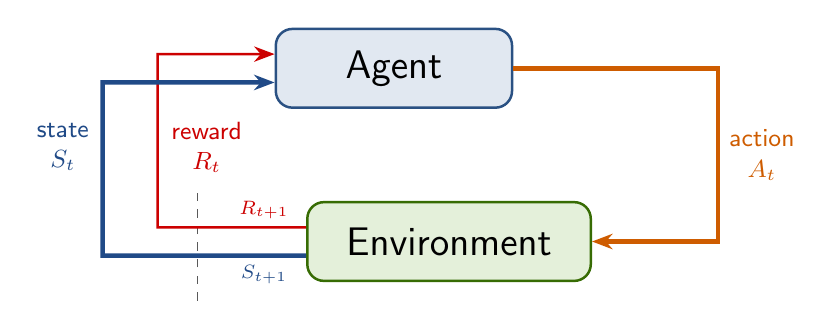
\begin{tikzpicture}[
    >={Stealth[length=2.6mm]},
    box/.style={draw, rounded corners=6pt, line width=0.9pt,
                minimum width=3.0cm, minimum height=1.0cm, font=\Large\sffamily},
    lbl/.style={font=\small\sffamily, align=center},
]
    \definecolor{agentc}{RGB}{52,101,164}
    \definecolor{envc}{RGB}{78,154,6}
    \definecolor{actc}{RGB}{206,92,0}
    \definecolor{statec}{RGB}{32,74,135}
    \definecolor{rewc}{RGB}{204,0,0}

    \node[box, fill=agentc!15, draw=agentc!80!black] (A) at (0,2.2) {Agent};
    \node[box, fill=envc!15,  draw=envc!70!black, minimum width=3.6cm] (E) at (0.7,0) {Environment};

    % action
    \draw[->, actc, line width=1.6pt]
        (A.east) -- ++(2.6,0) |- (E.east)
        node[pos=0.25, right, lbl, text=actc] {action\\ \(A_t\)};

    % dashed step boundary
    \draw[dashed, gray!70!black] (-2.5,-0.75) -- (-2.5,0.65);

    % reward (inner loop)
    \draw[->, rewc, line width=0.9pt]
        ([yshift=0.18cm]E.west) -- (-3.0,0.18) -- (-3.0,2.38) -- ([yshift=0.18cm]A.west);
    \node[lbl, text=rewc, anchor=west] at (-2.95,1.2) {reward\\ \(R_t\)};
    \node[font=\scriptsize, text=rewc] at (-1.65,0.40) {\(R_{t+1}\)};

    % state (outer loop)
    \draw[->, statec, line width=1.6pt]
        ([yshift=-0.18cm]E.west) -- (-3.7,-0.18) -- (-3.7,2.02) -- ([yshift=-0.18cm]A.west);
    \node[lbl, text=statec, anchor=east] at (-3.75,1.2) {state\\ \(S_t\)};
    \node[font=\scriptsize, text=statec] at (-1.65,-0.42) {\(S_{t+1}\)};
\end{tikzpicture}

    \caption{Agent--environment interaction loop in Reinforcement Learning.
    The agent selects an action \(A_t\), the environment evolves, and the
    next state \(S_{t+1}\) and reward \(R_{t+1}\) are fed back to the agent.}
    \label{fig:rl_loop}
\end{figure}
%
\noindent The standard formulation is a Markov Decision Process (MDP), defined by a state
space \(\mathcal{S}\), an action space \(\mathcal{A}\), transition dynamics
\(p(s_{t+1} \mid s_t, a_t)\), a reward function \(r(s_t,a_t)\), and a
discount factor \(\gamma \in [0,1)\). A stochastic policy
\(\pi_\theta(a_t \mid o_t)\) maps an observation to a probability
distribution over the available actions, rather than always selecting a
single fixed action. During training, this distribution allows the agent to
sample different actions and explore their outcomes. For discrete action
spaces, \(\epsilon\)-greedy selection offers a simple alternative: with
probability \(1-\epsilon\), the agent chooses the action with the highest
estimated value, and with probability \(\epsilon\), it chooses an action at
random. The aim of training is to find the parameter vector \(\theta^*\) that
maximises the expected discounted reward, or return,
%
\begin{equation}
    J(\theta) =
    \mathbb{E}_{\pi_\theta}
    \left[
        \sum_{t=0}^{T} \gamma^{t} r_t
    \right].
    \label{eq:rl_return}
\end{equation}
%
The discount factor determines the relative weight of future rewards. Values
close to one give greater weight to delayed consequences, whereas values close
to zero favour immediate rewards.\\
\
During training, value functions are used to estimate the expected return
associated with a state or with a state--action pair. These estimates help
reinforcement-learning algorithms assess the long-term consequences of
decisions, beyond the reward observed immediately. The state-value function
\(V^\pi(s)\) gives the expected discounted return from state \(s\) when the
agent follows policy \(\pi\). The action-value function \(Q^\pi(s,a)\) gives
the expected discounted return after taking action \(a\) in state \(s\) and
following \(\pi\) thereafter.
Their difference,
\(A^\pi(s,a)=Q^\pi(s,a)-V^\pi(s)\), is the advantage function: it measures whether
an action offers a higher or lower expected return than the policy's average
choice in that state.\\
\
In Value-based methods, the agent learns to estimate how much return can be expected from
each action in a given state, then use these estimates to choose an action.
Policy-gradient methods take a different route: they adjust the policy
parameters directly without optimizing a Value function.
In this setup, Actor--critic methods combine the two roles: an actor represents and updates
the policy, while a critic estimates value to guide those updates. In deep
RL, neural networks can approximate the policy, the value function, or both.\\
\
Proximal Policy Optimization (PPO) is a policy-gradient method commonly
implemented within an actor--critic framework \cite{ppo}. During training, the
actor updates the policy using sampled experience, while the critic learn a estimation of
the states and helping the actor to choose better actions. The policy update aims
to increase the likelihood of actions associated with higher estimated
returns. PPO's surrogate objective compares the current policy with the policy
that collected the data, using the probability ratio
\(\rho_t(\theta)=\pi_\theta(a_t \mid o_t)/
\pi_{\theta_{\mathrm{old}}}(a_t \mid o_t)\):
%
\begin{equation}
    L^{\mathrm{CLIP}}(\theta) =
    \mathbb{E}_t
    \left[
        \min\!\left(
            \rho_t(\theta)\,\hat{A}_t,\;
            \operatorname{clip}\!\left(\rho_t(\theta), 1-\epsilon, 1+\epsilon
            \right)\hat{A}_t
        \right)
    \right],
    \label{eq:ppo_clip}
\end{equation}
%
where \(\hat{A}_t\) is an estimated advantage and \(\epsilon\) sets the
range used to limit the incentive for large policy updates. The clipping term
reduces the incentive to move the updated policy too far from the one that
generated the sampled data, which is the old one.\\
\
In end-to-end RL, the policy learns the mapping from observations to the
selected action representation without requiring a separately designed planner
to provide intermediate decisions. This does not imply that every processing
or control stage is learned: observations can still be preprocessed, and a
low-level controller can convert policy outputs into actuator commands. The
observation and action spaces determine what information the agent can use and
which decisions it must learn.\\
\
Learning also requires a balance between exploration and exploitation. The
agent must try actions whose outcomes are uncertain while using its current
knowledge to obtain reward. The reward definition shapes this search, and the
training distribution determines which situations the agent encounters. A high
training return therefore does not establish that the policy will perform well
under different conditions. Generalisation must be evaluated separately. A
penalty in the reward can discourage undesirable behaviour, but it does not
guarantee that the learned policy will always satisfy the corresponding
requirement.



\newpage
\section{Residual Reinforcement Learning}

Residual Reinforcement Learning augments a baseline controller with a learned
policy that correct the output of the overall architecture. Given a state \(s_t\), the
baseline action and the learned residual determine the action applied to the
system:
%
\begin{equation}
    a_t =
    \pi_{\mathrm{base}}(s_t) + \pi_{\mathrm{residual}}(s_t),
    \label{eq:residual_policy}
\end{equation}
%
where \(\pi_{\mathrm{residual}}\) is the learned correction
\cite{residual_policy,residual_robot_control}. If the residual is initialized
to output zero, the robot initially behaves exactly like the baseline. The
policy therefore never starts from nothing, it inherits a controller that
already works, and only has to learn what that controller
gets wrong \cite{residual_policy}. This is especially useful for statically unstable
robots, where poor initial actions can quickly lead to a fall
\cite{hybrid_balance}.\\
\
A residual policy can be connected to the controller at
different levels: it can adjust the final actuator command
\cite{residual_mpc,hybrid_balance}, modify an internal model-based module
\cite{modular_residual,model_gap}, or provide high-level
decisions \cite{non_gaited}. These choices
assign different parts of the control task to learning and optimisation.\\
\
One way to combine learning with model-based control is to blend the policy
output with the controller output. In \cite{residual_mpc} three interfaces
for this correction are compared. In the first, the action \(a\) shifts
the joint-position setpoint produced by the MPC,
%
\begin{equation}
    \tau = K_p\left(q_{\mathrm{cmd}} + \lambda a - q\right)
    + K_d\left(\dot{q}_{\mathrm{cmd}} - \dot{q}\right) + \tau_{\mathrm{cmd}}.
    \label{eq:blend_joint_joint}
\end{equation}
%
In the second, the action specifies a joint target relative to a default pose
\(\hat{q}\). A PD law converts this target into a torque correction, which is
then added to the MPC torque,
%
\begin{equation}
    \tau_{\mathrm{res}} = K_p\left(a + \hat{q} - q\right) - K_d \dot{q},
    \qquad
    \tau = \tau_{\mathrm{MPC}} + \lambda \tau_{\mathrm{res}}.
    \label{eq:blend_joint_torque}
\end{equation}
%
In the third, the policy outputs a torque correction directly, which is added
to the MPC torque:
%
\begin{equation}
    \tau = \tau_{\mathrm{MPC}} + \lambda \tau_{\mathrm{RL}},
    \qquad \tau_{\mathrm{RL}} = \pi_\theta(o_t).
    \label{eq:blend_direct_torque}
\end{equation}
%
Here the learned action is added after the nominal optimisation rather than
being expressed as a reference for the lower-level controller. In
\cite{hybrid_balance}, the policy uses the same blending rule as
Eq.~\eqref{eq:blend_direct_torque}, adding its compensation torques to the
outputs of the balance and pose controller.\\
\
In TITA, the policy runs at \(100\)~Hz and contributes a residual correction
at the low-level control interface. The exact composition of the nominal and
residual torque terms is described in Section~\ref{subsec:tita_training_environment}.\\
\
Other hybrid architectures place learned corrections inside predictive
models or use a high-level policy to set motion commands and contact
sequences \cite{model_gap,modular_residual,adaptive_mpc,non_gaited,
deep_tracking}. In TITA, the nominal DFCIP-MPC handles the commanded motion
and its unicycle model directly tracks CoM velocity and wheel speed. Unlike
legged locomotion, where successive foot contacts can produce oscillations in
CoM velocity, the wheels provide continuous rolling motion: once they reach
their reference speed, the nominal controller can sustain the commanded
velocity without changing the high-level reference or contact sequence. A
high-level policy or modifications to the MPC modules are therefore not
needed for basic velocity tracking task.\\
\
The TITA nominal model assumes flat ground and continuous contact so,
if this assumptions is violated, the model may no longer accurately 
predict the system's behavior, which particularly 
matters for this platform in because the balance is inherently unstable.
The residual policy is intended
to improve robustness of locomotion through a low-level correction,
leaving the nominal controller responsible for tracking the commanded
motion.


\clearpage

\chapter{Hybrid MPC and Reinforcement Learning Architectures}

\section{Architecture Overview}

\section{Neural Network Design}

\section{Training Algorithm and Environment}
\label{subsec:tita_training_environment}


\clearpage

\chapter{Results}

\section{Simulation performances}
This is temporary content.

\section{Deployment on hardware}
This is temporary content.


\clearpage

\chapter{Conclusions}

This is temporary content.


\clearpage

\bibliographystyle{plain}
\bibliography{citations}

\end{document}
